\chapter{Fundamentos: Processos}

\begin{definicao}{Processo}
  É um programa em execução, composto por:
  \begin{itemize}
    \item Código em execução;
    \item Pilha de execução e seu apontador;
    \item Contado de programa (\texttt{PC});
    \item Valores de registradores de máquina;
    \item E outras informações.
  \end{itemize}
\end{definicao}

Cada processo possui um identificador único, conhecido como \textit{pid}. As informações do processo ficam armazenadas na \textbf{tabela de processos}, sendo o \textit{pid} seu indexador na tabela.

Durante a execução, o processo compartilha o processador com outros processos, sendo eles escalonados ao longo do tempo. A interação entre processos ocorre por mecanismos de comunicação próprios.

Por fim, existem dois escopos que carregam variáveis sobre a execução do processo:

\begin{itemize}
  \item \textbf{Ambiente:} contendo o espaço de endereçamento, arquivos abertos, processos filhos, sinais, estatísticas de uso, etc.;

  \item \textbf{Execução:} contendo registradores utilizados pelo processo, como o PC e o apontador de pilha, e o estado de execução do processo.
\end{itemize}


















\section{Modelo de Processos}
Classificamos os processos em relação ao custo de troca de contexto e manutenção:

\begin{itemize}
  \item \textbf{\textit{Heavyweight}:} são os processos tradicionais. Na sua entrada da tabela de processos temos tanto as informações de ambiente como as de execução;
  \item \textbf{\textit{Lightweight}:} são as \textit{threads}. Sua entrada na tabela de processos só contém informações de ambiente.
\end{itemize}

No modelo \textit{heaveweight}, também chamado de modelo tradicional, cada processo tem um único fluxo de controle, ou seja, em um dado momento ele só tem um valor de \texttt{PC}. Este processo roda independente dos demais e pode conter processos \textit{threads} que dependem dele.
% TODO: checar a última frase

Todo sistema operacional deve possuir mecanismos que permitam a criação de processos. Geralmente, um processo somente é criado por outro processo, o que nos leva uma \textbf{hierarquia de árvore de processos}. Entretanto, é necessário frisar que a árvore de processos não é de fato implementada. A partir do campo de ID do processo pai (PPID), podemos virtualmente implementar essa árvore. Implementá-la de fato seria muito custoso.






















\section{Estado do Processo}
Apesar de processos serem relativamente auto-suficientes, muitas vezes eles necessitam de acessar outros recursos (discos, terminais) ou mesmo se comunicar com outros processos. Quando um processo está ocioso, esperando que um evento aconteça, nós dizemos que ele está bloqueado. Em algumas situações, o processo pode ser bloqueado a revelia pelo sistema operacional. Podemos ter os seguintes estados:

Estados:
\begin{itemize}
  \item \textbf{Rodando:} processo em execução
  \item \textbf{Bloqueado:} processo parado, aguardando alguma coisa;
  \item \textbf{Pronto:} processo parado, pronto para ser executado, aguardando sua vez.
\end{itemize}

Usando a Figura \ref{fig:proc-states} como referências, podemos ilustrar as diversas passagens de estados ao longo da vida de um processo:

\begin{enumerate}
  \item O processo bloqueia-se à espera de um evento ou recurso;

  \item O evento ou recurso esperado pelo processo está disponível.Ele agora pode se executar, passando para o estado de \textit{Pronto};

  \item O processo é escolhido pelo escalonador para execução;

  \item O tempo de posse do processador pelo processo acabou. O SO retira o processador do processo.
\end{enumerate}

\begin{figure}[ht]
  \centering
  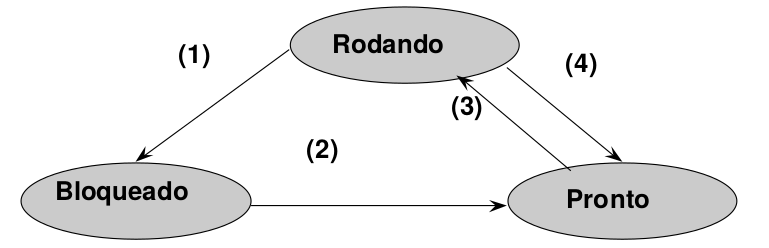
\includegraphics[width=.75\textwidth]{proc-states}
  \caption{Possíveis estados de um processo.}
  \label{fig:proc-states}
\end{figure}

















\section{Tabela de Processos}
\begin{definicao}{Tabela de Processos}
  Estrutura que contem os todas as informções relativas à manutenção de cada processo do SO, guardando os campos de gerência de processos, memória e arquivos. Possui uma entrada para cada processo.
\end{definicao}

Em relação a \textbf{gerência de processos}, as informações guardadas normalmente são: \textit{pid}, valor dos registradores de execução e PC, valor da palavra de estado, valor do apontador de pilha, estado do processo, instante do início do processo, tempo de processador utilizado e outros.

Em relação a \textbf{gerência de memória}, são guardados o endereço do segmento de texto, dados e pilha, sendo estes mandatórios. Podemos ter também estado da saída, informações sobre proteção e outros. Note que o segmento de texto é a porção de código do processo, que normalmente é \textit{read only}. Alguns sistemas com área de memória pequena tornam essa área \textit{read-write}, para uso eficiênte da memória, porém essa estratégia oferece riscos de segurança.

Em relação a \textbf{gerência de arquivos}, são guardados o diretório raíz e de trabalho, descritores de arquivos abertos, parâmetros de chamadas em andamentos e outras.




\subsection{Troca de Contexto}
\begin{definicao}{Contexto}
  No que diz respeito a processos, o contexto será o conjunto de valores dos registradores do processo.
\end{definicao}

Dessa forma, define-se a troca de contexto como a operação de salvamento dos registradores de um processo, para restauração dos conjunto de registradores de outro processo. Tal operação permite que haja a efetiva troca de processos no processador.




















\section{Escalonamento de Processos}
O algoritmo de escalonamento de processos é o responsável pela determinação de que processo, dentro do conjunto de processos prontos, vai rodar e por quanto tempo. Quando um processo solicita operações blocantes, sua execução fica suspensa até que o evento solicitado ocorra.

% TODO: dar exemplo de operações blocantes. Ex: I/O, load/store memória(?), perguntar +

Para garantir um bom algoritmo de escalonamento, alguns \textbf{critérios} devem ser seguidos:
\begin{itemize}
  \item \textbf{\textit{Fairness}:} garantir que todos os processos do sistema terão chances de uso do processador, ou seja, \textbf{não há \textit{starvation}}. Garantir que os processos tenham chances \textit{iguais}, é algo muito forte e não usamos essa definição;

  \item \textbf{Eficiência:} se há demanda, a CPU deve estar ocupada;

  \item \textbf{Minimizar o tempo de resposta:} % TODO: ver o que é isso

  \item \textbf{Minimizar o \textit{waiting time}:} ou seja, o tempo de resposta entre os estados \textit{Ready} e \textit{Running};

  \item \textbf{Maximizar o \textit{thoughtput}:} aumentar o número de processos conclúidos em um determinado tempo.
\end{itemize}

\begin{definicao}{Preempção}
  Suspensão temporária da execução de um processo.
\end{definicao}

Podemos classificar escalonadores segundo sua preempção:

\begin{itemize}
  \item \textbf{Escalonadores não-preemptivos:} quando um processo obtém o processador, ele roda até o seu fim ou até que ele peça uma operação blocante.

  Isto simplifica o projeto do escalonador, porém permite que o processo detenha a CPU por tempo arbitrário, levando-o ao monopólio do processador. Isto acaba por violar todos os critérios de um bom escalonador;

  \item \textbf{Escalonadores preemptivos:} cada processo possui um tempo máximo de permanência, chamado \textbf{\textit{quantum}}, de posse do processador. Quando o \textit{quantum} termina, o SO retira o processador deste processo, para permitir a execução de outro processo.

  Desta forma, estes escalonadores garantem um uso mais balanceado da CPU, o que levam a eles serem usados na maioria dos SOs. Entretanto, seu projeto é consideravelmente mais complexo, uma vez que os processos devem proteger suas regiões críticas de outros processos concorrentes.
\end{itemize}

\begin{definicao}{Região Crítica}
  Área que contém as estrutura de dados importantes de um processo em execução, não podendo ser acessada por concorrentemente, mas sim atômicamente.
\end{definicao}

O tempo de execução do processo é controlado por um \textit{clock} que gera interrupções em uma determinada frequência, chamadas de \textit{clock tick}. Tal ferramenta está presente em qualquer processador moderno.

O SO mantem um contador que é decrementado a cada \textit{clock tick}. Quando este contador chega a zero, o tempo de permanência do processo acabou e ele será retirado do processador. O valor inicial deste contador corresponde ao tempo máximo de permanência do processo com a CPU, denominado, \textbf{\textit{time slice}}.

Dado isto, podemos listar as \textbf{políticas de algoritmos de escalonamento} existentes.



\subsection{\textit{First Come First Served}}
Os processos que solicitam a CPU são colocados em uma fila \textit{ready}, gerênciada segundo a política FCFS: o primeiro processo que entrar, será o primeiro a ser executado por completo. Desta forma, é importante notar que este algoritmo é \textbf{não-preemptivo}.

\begin{figure}
  \centering
  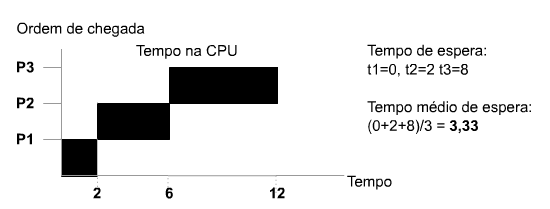
\includegraphics[width=0.75\textwidth]{scale-fcfs}
  \caption{Execução de processos em política FSFC com ordem chegada P1, P2 e P3.}
  \label{fig:scale-fcfs}
\end{figure}





\subsection{\textit{Round Robin}}
Cada processo tem o direito de usar o processador por um intervalo de tempo pré-definido, denominado \textbf{\textit{quantum}}. Quando este intervalo se esgota, o processador é dado a outro processo e o processo retirado vai para o fim da fila de processos. É versão preemptiva da política FSFC, sendo um algoritmo justo.





\subsection{Escalonamento com Prioridades}
Baseia-se no fato de que alguns processos são prioritários e, assim, devem ser executados antes dos outros. A cada processo é atribuída uma prioridade e os que tem maior prioridade são executados primeiro.

A prioridade pode ser definida de duas formas:
\begin{itemize}
  \item \textbf{Estaticamente:} os processos são divididos em classes e a cada classe é atribuída uma prioridade. A cada prioridade, existe uma fila de prontos associada. A política nas filas pode ser arbitrária;

  \item \textbf{Dinâmicamente:} o sistema analisa o comportamento dos processose atribui prioridades favorecendo um certo tipo de comportamento. Por exemplo, processos com I/O podem ter prioridades altas. O cálculo da prioridade pode ser dado por $1/f$, onde $f$ é a fração do \textit{quantum} de tempo utilizado na última rodada do processo.
\end{itemize}

 Note que é possível que um processo pode monopolizar a CPU caso ele precise de muito tempo de processamento e sua prioridade for a maior de todas. % TODO: isso ocorre tanto estaticamente como dinamicamente?






\subsection{\textit{Shortest Job First}}
Aqui, dado um conjunto de \textit{jobs} prontos, executamos os \textit{jobs} com menor tempo de execução antes.

Note que este algoritmo pode não ser muito justo, pois, supondo um processo com uma dada prioridade, este pode entrar em \textit{starvation} se todo novo processo que entrar na fila tiver tempo de execução menor que ele.























\section{\textit{Threads}}


\section{\textit{Deadlock}}
\begin{definicao}{\textit{Deadlock}}
  Um conjunto de processos está em \textit{deadlock} se cada processo pertencente ao conjunto estiver esperando por um evento que somente um outro processo pertencente ao mesmo conjunto pode fazer ocorrer. Ou seja, \textbf{é uma espera eterna por recursos}.
\end{definicao}

\begin{definicao}{\textit{Livelock}}
  ocorre quando um conjunto de processos estão em parte de sua execução que é um loop eterno do qual nunca saírão, geralmente fazendo \textit{pooling}
\end{definicao}

\textbf{Nota:} Do ponto de vista teórico, livelock e deadlock tem significados equivalentes.

\begin{definicao}{\textit{Starvation}}
  Ocorre quando um conjunto de processos é indefinidamente preterido porque sua prioridade é menor que a prioridade outros conjuntos de processos. Ou seja, é \textbf{uma espera por um tempo indefinido por recursos}.
\end{definicao}










\section{Comunicação entre Procesos}
Processos interagem entre si, trocando informações. Dito isso, temos dois tipos de trocas de informações, ou cooperações: por compartilhamento de variáveis ou por troca de mensagens.

\subsection{Compartilhamento de Variáveis}
Um processo escreve um valor em uma posição de memória e outro processo lê este mesmo valor. Como o sistema operacional determina, através da política de escalonamento, o processo que vai rodar e por quanto tempo, não sabemos a priori em
que ordem dois processos ativos irão se executar. Daí, podemos ter inconsistências. % TODO: pegar imagem do slide

\begin{definicao}{Condição de Corrida}
  Quando dois ou mais processos acessam concorrentemente as mesmas posições de memória e o valor final contido nestas posições \textbf{dependem da ordem} na qual os processos foram executados, então temos uma condição de corrida.
\end{definicao}

Condição de corrida pode não ser um erro ou algo indesejável. Alguns programadores podem tirar proveito disso. Além disso, podemos definir que os processos escrevam na mesma posição, porém forçando ser o mesmo valor. Neste último caso, \textit{não temos condição de corrida}.


\subsection{Exclusão Mútua}
Para evitar as condições de corrida, devemos estabelecer que os processos sejam executados segunda certa ordem, de maneira exclusiva.

\subsubsection{Espera Ocupada}

\subsubsection{Bloqueio de Processos}
